% =============================================================================
%  VI. RESULTS: INTERNAL TEMPORAL PERFORMANCE   
% =============================================================================
\begin{frame}{VI. Results: Internal Temporal Performance (Variant B)}
\begin{center}\tablestyle\footnotesize
\begin{tabular}{lllrr}
\toprule
\textbf{Model} & \textbf{AUROC} & \textbf{95\% CI}
  & \textbf{Utility (best)} & \textbf{Alert burden at best} \\
\midrule
Primary & \textbf{\pcAurocPrimaryB} & [\pcAurocCiLoPrimaryB, \pcAurocCiHiPrimaryB] & \pcUtilityMaxPrimaryB & \pcUtilityOptBurdenPrimaryB \\
GBT     & \pcAurocGbtB     & [\pcAurocCiLoGbtB, \pcAurocCiHiGbtB]         & \pcUtilityMaxGbtB     & \pcUtilityOptBurdenGbtB \\
Cox     & \pcAurocCoxB     & [\pcAurocCiLoCoxB, \pcAurocCiHiCoxB]         & \pcUtilityMaxCoxB     & \pcUtilityOptBurdenCoxB \\
NEWS2   & \pcAurocNewsB    & [\pcAurocCiLoNewsB, \pcAurocCiHiNewsB]       & \pcUtilityMaxNewsB    & \pcUtilityOptBurdenNewsB \\
SIRS    & \pcAurocSirsB    & [\pcAurocCiLoSirsB, \pcAurocCiHiSirsB]       & \pcUtilityMaxSirsB    & \pcUtilityOptBurdenSirsB \\
qSOFA   & \pcAurocQsofaB   & [\pcAurocCiLoQsofaB, \pcAurocCiHiQsofaB]     & \pcUtilityMaxQsofaB   & \pcUtilityOptBurdenQsofaB \\
\bottomrule
\end{tabular}
\end{center}
{\scriptsize Temporal test set, 2017--2019: \pcNTestRowsB{} person-hours and
\pcNTestEventsB{} onsets. Utility (best): maximised over the threshold grid;
$\infty$: no alert was optimal. Benchmark burden: 1.4~\cite{moor2023review}.\par}

\vspace{4pt}
\begin{itemize}\itemsep2pt\small
  \item The paired comparison favoured the primary model over GBT by
        \pcHSixAbsEst{} AUROC (H6). Both had higher AUROC than Cox, NEWS2, SIRS
        and qSOFA.
  \item Primary-model calibration slope: \pcCalibSlopePrimaryB{} (ideal = 1).
  \item AUROC in the mid-to-high 0.7s did not translate into a plausible
        alert burden: the best utility of the primary model and GBT required
        \pcUtilityOptBurdenPrimaryB{} and \pcUtilityOptBurdenGbtB{} false alerts
        per true alert.
\end{itemize}
\end{frame}


% =============================================================================
%  VI. RESULTS: AUROC VARIATION ACROSS ANALYSIS CHOICES
% =============================================================================
\begin{frame}{VI. Results: AUROC Variation Across Analysis Choices}
\begin{center}\renewcommand{\arraystretch}{1.1}\small
\begin{tabular}{p{6.4cm}cll}
\toprule
\textbf{Factor varied (others fixed)} & \textbf{$\Delta$AUROC} & \textbf{95\% CI} & \textbf{H} \\
\midrule
Model class (label B, temporal)       & \textbf{\pcSpreadModelClass} & [\pcSpreadModelClassCiLo, \pcSpreadModelClassCiHi] & n/a \\
Internal $-$ external (primary, label B) & \pcSpreadMetric     & [\pcHFiveCiLo, \pcHFiveCiHi] & H5 \\
Label definition (primary, temporal)  & \pcSpreadLabel      & [\pcSpreadLabelCiLo, \pcSpreadLabelCiHi] & H1 \\
Random $-$ temporal split (primary, label B) & \pcSpreadSplit      & [\pcHFourCiLo, \pcHFourCiHi] & H4 \\
\midrule
GBT $-$ primary (label B, temporal)   & \pcHSixEst          & [\pcHSixCiLo, \pcHSixCiHi] & H6 \\
\bottomrule
\end{tabular}
\end{center}
{\scriptsize These are ranges or contrasts, not additive variance components.
The model-class range covers six specifications and the label range three
definitions, so the two are not directly symmetric. The GBT--Cox difference
alone (\pcAurocGbtB{} vs \pcAurocCoxB) is about eight times the full label
range.\par}

\vspace{4pt}
\begin{itemize}\itemsep2pt\small
  \item \textbf{Model class} produced the largest AUROC range.
  \item The external contrast was second largest but imprecisely estimated:
        its interval includes zero.
  \item \textbf{Label and split effects were small} in this analysis.
\end{itemize}
\end{frame}


% =============================================================================
%  VI. RESULTS: CONFIRMATORY HYPOTHESES
% =============================================================================
\begin{frame}{VI. Results: Confirmatory Hypotheses (Holm-Corrected)}
\begin{center}\renewcommand{\arraystretch}{1.15}\scriptsize
\begin{tabular}{llrlr>{\raggedright\arraybackslash}p{3.7cm}}
\toprule
\textbf{H} & \textbf{Contrast} & \textbf{Est.} & \textbf{95\% CI}
  & \textbf{$p_{\text{Holm}}$} & \textbf{Verdict} \\
\midrule
H1 & Label spread $-$ model spread  & \pcHOneEst & [\pcHOneCiLo, \pcHOneCiHi] & \pcHOnePHolm & \pcHOneVerdict \\
H2 & Unstable covariates (count)    & \pcHTwoEst & n/a & n/a & Descriptive \\
H3 & Pre-treatment onsets (count)   & \pcPreTreatOnsetsVarB & n/a & n/a & Definitional \\
H4 & Random $-$ temporal AUROC      & \pcHFourEst & [\pcHFourCiLo, \pcHFourCiHi] & \pcHFourPHolm & \pcHFourVerdict \\
H5$^{\dagger}$ & Internal $-$ external AUROC & \pcHFiveEst & [\pcHFiveCiLo, \pcHFiveCiHi] & \pcHFivePHolm & \pcHFiveVerdict \\
H6 & GBT $-$ primary AUROC          & \pcHSixEst & [\pcHSixCiLo, \pcHSixCiHi] & \pcHSixPHolm$^{\ddagger}$ & \pcHSixVerdict \\
\bottomrule
\end{tabular}
\end{center}
{\tiny $^{\dagger}$Post-hoc substitute: internal utility was too close to zero
for a proportional decline to be defined, so an AUROC contrast takes its
place.
$^{\ddagger}$Tests the pre-registered interval null $|\theta| \leq 0.02$;
non-inferiority is read from the confidence interval, not from this p-value.\par}

\vspace{2pt}
\begin{itemize}\itemsep0pt\footnotesize
  \item \textbf{H1 not confirmed:} model spread \pcSpreadModelClass{} vs label
        spread \pcSpreadLabel; opposite direction, interval excludes zero.
  \item \textbf{H4 not confirmed:} random-split AUROC was \pcHFourAbsEst{}
        \emph{lower} than temporal (\pcAurocRandomPrimaryB{} vs
        \pcAurocPrimaryB); the interval includes zero.
  \item \textbf{H6:} GBT $-$ primary $= \pcHSixEst$; the upper limit
        (\pcHSixCiHi) lies below the $+0.02$ margin, supporting one-sided
        \textbf{non-inferiority}, not two-sided equivalence.
\end{itemize}
\end{frame}


% =============================================================================
%  VI. RESULTS: H3, THE PRE-TREATMENT WINDOW
% =============================================================================
\begin{frame}{VI. Results: Why H3 Was Not Evaluable}
\vspace*{0pt}%
{\footnotesize Status: \notevaluable. The pre-registered onset rule produced no
pre-treatment onsets, so the contrast could not be formed.\par}
\begin{block}{Structural reason}
  \footnotesize In Variants A, B, C and E, onset is assigned to the
  \emph{later} event of the antibiotic--culture pair, so onset cannot precede
  the treatment anchor. The window is empty \textbf{by definition}, not
  because no events were observed.
\end{block}

\vspace{2pt}
\begin{center}\tablestyle\footnotesize
\begin{tabular}{llrrl}
\toprule
\textbf{Var} & \textbf{Label} & \textbf{Pre-treatment person-h}
  & \textbf{Onsets} & \textbf{AUROC (primary / GBT)} \\
\midrule
B & Seymour-Std   & \pcPreTreatPersonHoursVarB & \textbf{\pcPreTreatOnsetsVarB} & undefined \\
F & Sepsis-3 Early-Onset & \pcPreTreatPersonHoursVarF & \textbf{\pcPreTreatOnsetsVarF}
  & \pcPreTreatAurocPrimaryF{} / \pcPreTreatAurocGbtF \\
D & Deterioration & \pcPreTreatPersonHoursVarD & \textbf{\pcPreTreatOnsetsVarD}
  & \pcPreTreatAurocPrimaryD{} / \pcPreTreatAurocGbtD \\
\bottomrule
\end{tabular}
\end{center}

\begin{itemize}\itemsep1pt\footnotesize
  \item \textbf{Variant F} (post-hoc) keeps B's cases but uses the standard
        earlier onset, $\min(t_{\text{susp}}, t_{\text{SOFA}})$. It moves
        \pcFNMovedEarlier{} of \pcFNOnsets{} onsets earlier (median shift
        \pcFMedianShiftH\,h), \pcFNBeforeAnchorTest{} of them into the
        test-set pre-treatment window.
  \item The concern about treatment-dependent case
        membership~\cite{kamran2024evaluation} remains relevant; its effect on
        onset timing depends on the onset rule. These AUROCs assess detection
        at the assigned onset, not advance prediction.
\end{itemize}
\end{frame}


% =============================================================================
%  VI. RESULTS: LABEL-ANCHOR ATTRIBUTION        
% =============================================================================
\begin{frame}{VI. Results: Post-Hoc Decomposition of the Sepsis-3 Label}
\vspace*{0pt}%
{\footnotesize Labels D, E and F are post-hoc protocol amendments: \exploratory\par}
\begin{atucols}[c]
\begin{column}{0.52\textwidth}
  \centering
  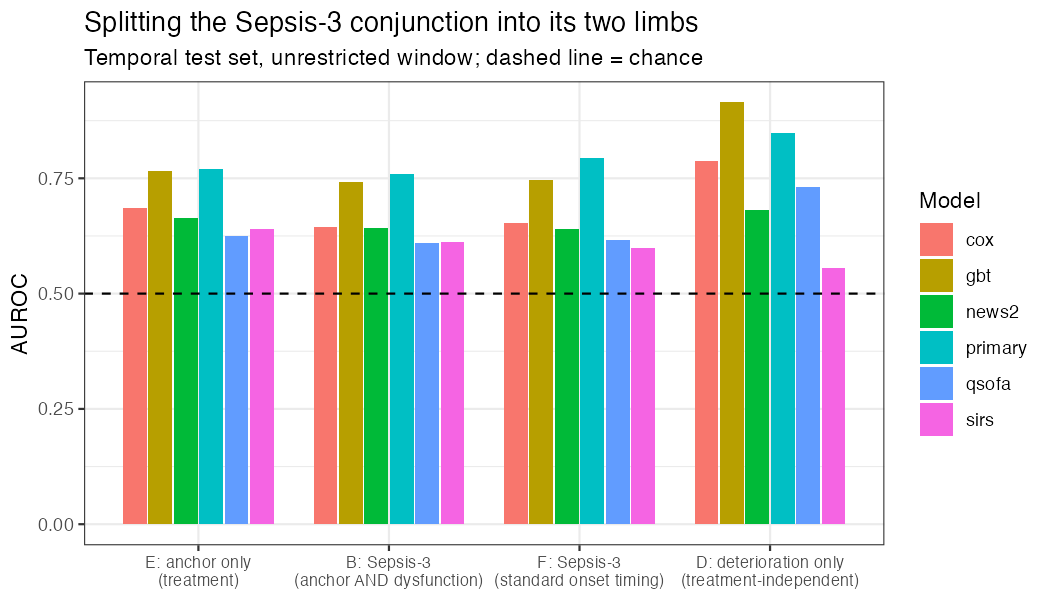
\includegraphics[width=\columnwidth]{images/09_label_anchor_attribution.png}
\end{column}
\begin{column}{0.46\textwidth}
\begin{itemize}\itemsep1pt\scriptsize
  \item \textbf{E (Anchor-Only)} removes SOFA but keeps B's onset hour in
        \pcPctExactMatchE\% of B's cases: SOFA affects membership, not onset
        time.
  \item Anchor-attributable fraction $\phi_{\text{anchor}}$: primary
        \pcPhiAnchorPrimary{} [\pcPhiAnchorCiLoPrimary,
        \pcPhiAnchorCiHiPrimary]; GBT \pcPhiAnchorGbt{} [\pcPhiAnchorCiLoGbt,
        \pcPhiAnchorCiHiGbt].
  \item \textbf{D (Deterioration)} removes treatment timestamps; agreement
        with B is low ($\kappa = \pcKappaVsBD$). Five of its six SOFA
        components are model inputs, so its AUROC is partly
        self-fulfilling.
  \item \textbf{F (standard onset timing):} primary AUROC
        \pcAurocPrimaryB{} $\rightarrow$ \pcAltAurocFullPrimaryF; the GBT
        change was small and not statistically detectable
        ($\Delta = \pcAltDeltaGbtF$, $q = \pcAltDeltaPBhGbtF$).
\end{itemize}
\end{column}
\end{atucols}

\vspace{2pt}
\begin{alertblock}{}
  \footnotesize For the primary model, onset timing had a larger effect than
  removing SOFA. No corresponding timing effect was detected for GBT.
\end{alertblock}
\end{frame}


% =============================================================================
%  VI. RESULTS: UTILITY CEILING             
% =============================================================================
\begin{frame}{VI. Results: Clinical Utility Across Alert Thresholds}
\begin{center}
  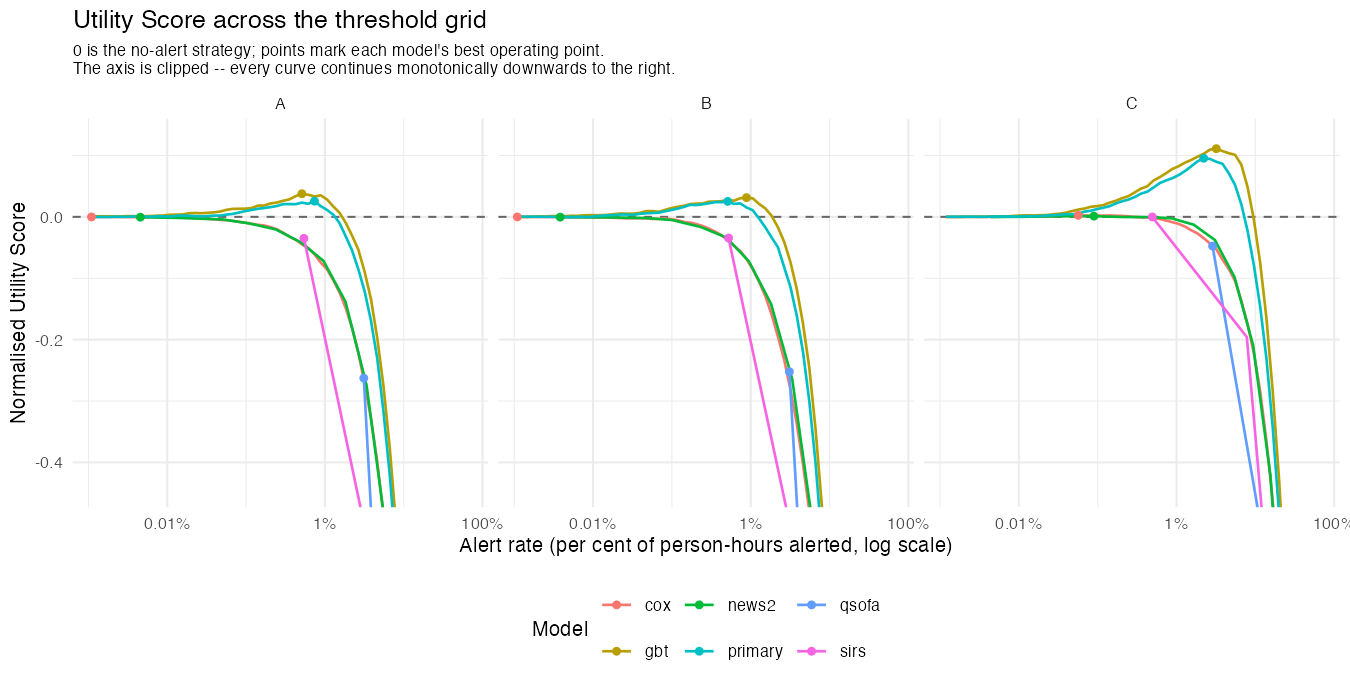
\includegraphics[width=\textwidth,height=0.53\textheight,
                   keepaspectratio]{images/07_utility_threshold_sweep.png}
\end{center}
\vspace{-4pt}
\begin{itemize}\itemsep1pt\footnotesize
  \item At the 0.5 threshold the primary model issued no alerts, so its
        utility was \pcUtilityPrimaryB.
  \item Across all models and thresholds, the highest Variant B utility was
        \textbf{\pcUtilityMaxGbtB{} (GBT)}, at \textbf{\pcUtilityOptBurdenGbtB{}
        false alerts per true alert} (benchmark: 1.4~\cite{moor2023review});
        under any pre-registered variant, \pcUtilityMaxGbtC{} (GBT, C).
  \item Thresholds were selected on the test set, so these maxima are
        optimistic.
\end{itemize}
\end{frame}


% =============================================================================
%  VI. RESULTS: EXTERNAL VALIDATION ON eICU-CRD   
% =============================================================================
\begin{frame}{VI. Results: External Validation Limited by Label Observability}
\begin{center}\tablestyle\footnotesize
\begin{tabular}{lrrrrr}
\toprule
\textbf{Var} & \textbf{Internal (primary)} & \textbf{eICU primary}
  & \textbf{eICU GBT} & \textbf{eICU NEWS2} & \textbf{eICU events} \\
\midrule
A & \pcAurocPrimaryA & \pcExtAurocPrimaryA & \pcExtAurocGbtA & \pcExtAurocNewsA & \pcExtNEventsA \\
B & \pcAurocPrimaryB & \pcExtAurocPrimaryB & \pcExtAurocGbtB & \pcExtAurocNewsB & \pcExtNEventsB \\
C & \pcAurocPrimaryC & \pcExtAurocPrimaryC & \pcExtAurocGbtC & \pcExtAurocNewsC & \pcExtNEventsC \\
\bottomrule
\end{tabular}
\end{center}
{\scriptsize eICU microbiology-covered subset; frozen models, no
retraining.\par}

\vspace{2pt}
\begin{itemize}\itemsep1pt\footnotesize
  \item Culture data covered \textbf{\pcExtMicroCoverage\% of eICU cohort
        stays}, leaving \pcExtNEventsB{} Variant B events, below the
        \pcExtMinEvents-event interpretability floor.
  \item H5 substitute, internal $-$ external AUROC $= \pcHFiveEst$
        [\pcHFiveCiLo, \pcHFiveCiHi]: the point estimate is lower externally,
        but the interval includes zero, so the contrast is inconclusive. The
        source of the difference was not identified.
  \item Antibiotic-only (\pcExtAbxNEventsB{} events) and Variant D
        (\pcExtAltNEvents{} events) analyses had more events but measure
        different targets; both showed lower external discrimination.
\end{itemize}
\end{frame}


% =============================================================================
%  VI. RESULTS: H2, ABLATION AND EQUITY      
% =============================================================================
\begin{frame}{VI. Results: Coefficient Instability and Subgroup Analysis}
\begin{atucols}[t]
\begin{column}{0.49\textwidth}
\begin{block}{H2: coefficient instability (descriptive)}
\begin{itemize}\itemsep1pt\scriptsize
  \item \pcHTwoEst{} of \pcHTwoNTerms{} covariates met the instability rule:
        \pcHTwoNSign{} by sign, \pcHTwoNMag{} by $\geq 2$-fold magnitude
        (categories overlap).
  \item \textbf{After accounting for estimation uncertainty, \pcHTwoNRobust{}
        remained unstable, all test-order
        indicators}~\cite{lauritsen2021framing}. The raw count is an upper
        bound on the instability present.
  \item \textbf{Ablation} (post-hoc): removing the \pcAblNDropped{}
        action-derived covariates reduced instability from \pcHTwoEst/\pcHTwoNTerms{}
        to \pcAblHTwoNUnstable/\pcAblHTwoNTerms{} and changed AUROC by
        \pcAblDeltaAurocPrimaryB{} \pcAblDeltaCiPrimaryB{} (primary, B):
        small, but not absent.
\end{itemize}
\end{block}
\end{column}
\begin{column}{0.49\textwidth}
\begin{block}{Label sensitivity by recorded subgroup (exploratory)}
\begin{itemize}\itemsep1pt\scriptsize
  \item Subgroup AUROC: \pcEquityNContrastsEOne{} contrasts met the
        100-event requirement; \textbf{none remained significant} after BH
        correction.
  \item Only two race categories met it, one of them \emph{Unknown}, so no
        adequately powered comparison between two recorded categories was
        available.
  \item Label sensitivity: the only racial strata above the White reference
        are \emph{Unknown} ($+\pcLabelSensUnknownPp$\,pp,
        $q = \pcLabelSensUnknownQ$) and \emph{Unable to obtain}
        ($+\pcLabelSensUnablePp$\,pp, $q = \pcLabelSensUnableQ$), both
        \textbf{missingness categories}.
  \item This may reflect record completeness, a mechanism not
        tested~\cite{wang2022equity}; no stratum recording an actual answer
        differs from the reference.
\end{itemize}
\end{block}
\end{column}
\end{atucols}
\end{frame}
